\renewcommand\maketitle{
{
    \setlength{\unitlength}{0.1\paperheight}
    \setbeamertemplate{background canvas}{%
        \color{white}%
        \begin{picture}(10,10)%fond
            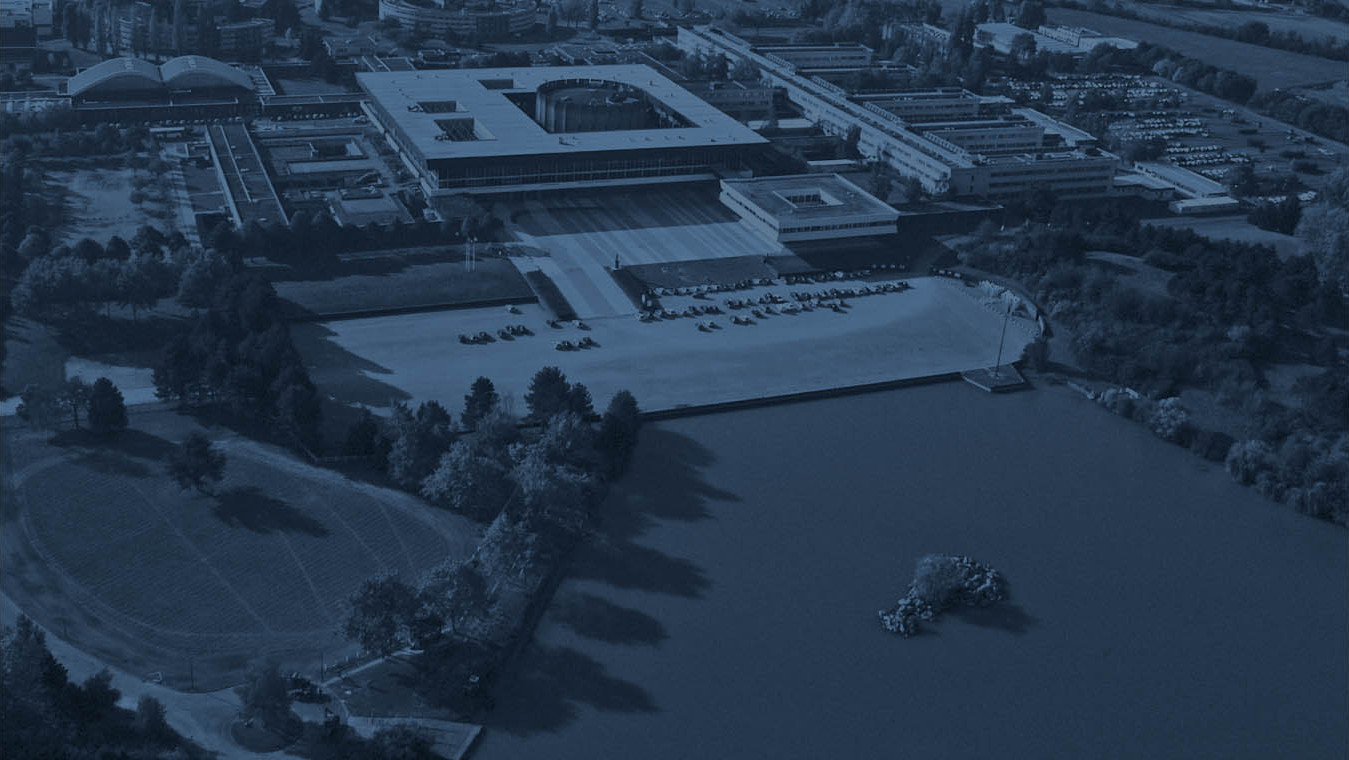
\includegraphics[height=\paperheight,keepaspectratio]{img/fond_ecole}%
        \end{picture}%
        \hspace*{-\paperheight}%
        \begin{picture}(3,10)%date
            \setlength{\unitlength}{1ex}%
            \put(0.5,0.5){\footnotesize \polydatesave}%
        \end{picture}%
        \begin{picture}(3,10)%auteur
            \setlength{\unitlength}{1ex}%
            \put(0.5,0.5){\footnotesize \polyauteursave}%
        \end{picture}
        \hspace*{-0.6\paperheight}
        \tikz\node[remember picture, overlay, right] at (current page.west) {
\includegraphics[height=0.33\paperheight]{img/whitelogo}};
    }
    \begin{frame}[plain,c]
        \color{white}
        \begin{flushright}
            \begin{picture}(9,6)
                \put(0,2.95){%titre
                    \makebox(9,3.05)[br]{%
                        $\text{%
                            \bfseries\begin{minipage}{9\unitlength}%
                                \Large\setlength{\baselineskip}{0.7\baselineskip}%
                                \begin{flushright}%
                                    \polytitresave%
                                \end{flushright}%
                            \end{minipage}%
                        }$%
                    }%
                }
                \put(0,0){%sous-titre
                    \makebox(9,2.75)[tr]{%
                        $\text{%
                            \begin{minipage}{9\unitlength}%
                                \setlength{\baselineskip}{0.7\baselineskip}%
                                \begin{flushright}%
                                    \polysoustitresave%
                                \end{flushright}%
                            \end{minipage}%
                        }$%
                    }%
                }
            \end{picture}
        \end{flushright}
    \end{frame}
}
}
\setbeamertemplate{background canvas}{}